% PREAMBLE

\documentclass[norsk]{article}
\usepackage[utf8]{inputenc}
\usepackage[T1]{fontenc}
\usepackage{graphicx}
\usepackage{float}
\usepackage[sc]{mathpazo}
\linespread{1.05}
\usepackage{latexsym}
\usepackage{hyperref}
\tolerance=1000
\usepackage[T1]{fontenc}
\setlength{\parindent}{0.0in}
\setlength{\parskip}{0.0in}
\usepackage{setspace}
\onehalfspacing
\usepackage[raggedright,bf,sf]{titlesec}
\usepackage{fullpage}
\usepackage{xcolor}
\usepackage{listings}
\renewcommand{\maketitle}{}
\usepackage[norsk]{babel}

\definecolor{lightgray}{gray}{0.95}
\lstnewenvironment{code}[1][]%
  {\minipage{\linewidth}
\lstset{
  language=,
  keywordstyle=\bfseries,
  captionpos=b,
  backgroundcolor=\color{lightgray},
  frame=shadowbox,
  rulesepcolor=\color{gray},
  basicstyle=\ttfamily\fontsize{10}{10}\selectfont,
  aboveskip=20pt,
  #1}}
  {\endminipage}

% DOCUMENT
\begin{document}

\maketitle

\newcommand{\blankpage}{\newpage{}\thispagestyle{empty}\mbox{}\newpage{}}
\newcommand{\HRule}{\rule{\linewidth}{0.5mm}}

\begin{titlepage}
\begin{center}

\includegraphics[width=8cm]{uib-emblem-svart} \\[0.5cm]
\paragraph*{}

\textsc{\Large Informasjonsvitenskap}\\[0.5cm]
\Large INFO 233, Vår 2014\\[0.4cm]
\HRule \\[0.4cm]
{ \huge \bfseries Andre Obligatoriske oppgave}\\[0.5cm]
\HRule \\[1.0cm]

{\large \emph{Utlevert 18.mars 2014}}\\
{\large \emph{Innleveringsfrist klokken 15.00, 7. mai 2014}}\\



\paragraph*{}
\end{center}
\vfill
\begin{center}
\end{center}
\end{titlepage}

\blankpage

\section{Regler}
\label{sec:regler}
Oppgaver vurderes til godkjent/ikke godkjent.\\
Dere jobber enkeltvis eller i par.\\
%brukernavn på fil og prosjektnavn.
Leveringsformatet er et Eclipseprosjekt, eksportert til en komprimert fil. (En av: zip, tgz eller tar.gz. Rar-filer godtas ikke.)\\ % Vi kan per lov ikke kommunisere i proprietære formater som rar.
Merk at prosjektet dere får utlevert er i UTF-8. Dere bør derfor etter å ha importert det, sjekke filformatet. Det gjør dere ved å høyreklikke på prosjektmappen, velge properties, og passe på at det ser ut som dette:
\begin{figure}[h!]
  \centering
    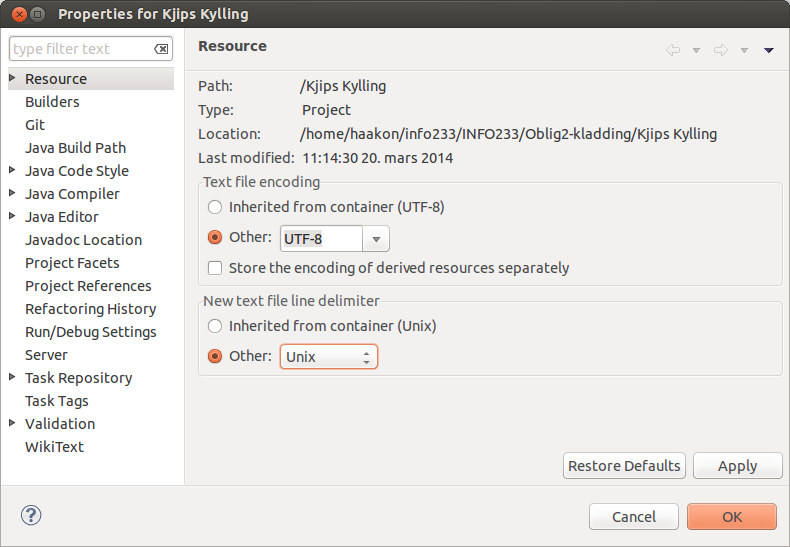
\includegraphics[width=1\textwidth]{slik-ser-det-ut.png}
\end{figure}


\section{Oppgaven}
\label{sec:oppgaven}
Den andre obligen omhandler en utvidelse av et spill, kalt Kjips Kylling, som er en forenklet klon av Chip's Challenge\footnote{Se \url{http://en.wikipedia.org/wiki/Chip\%27s_Challenge} for mer om spillet}.
Spillet har allerede en enkel grafikkmotor, og dere skal utvide spillet.
Lyd er ikke en del av obligen, og dere kan ignorere alt som har med lyd å gjøre. % Skal vi nevne dette til å begynne med, eller vente til de spør på gruppene?

Før dere begynner å kode anbefaler vi å lese godt igjennom oppgaven, se hvordan relevante kodebiter fungerer, og tenke gjennom før en begynner å kode.
Husk å bruke tiden godt. Det er nok å gjøre, og mye blir lettere å gjøre hvis dere har en plan først. % Jeg kan ikke si dette mange nok ganger, men jeg tror jeg gjør et forsøk her. ^_^;

\section{Spillet}
\label{sec:spillet}
Spillet Kjips Kylling består av flere brett, en spiller og monstre.
Målet med spillet er å klare alle brettene.
For å klare et brett må du komme deg fra begynnelsen på brettet til slutten.
Dersom du går tom for tid, kommer borti et monster, eller tråkker på en dødelig rute i spillet dør du.
Når du dør kan du prøve brettet på nytt.
Brettet består av forskjellige ruter. Noen kan gås på, andre ikke. Noen er dødelige, andre ikke.
Brettet har også forskjellige monstre. Disse monstrene beveger seg etter faste mønstre. Monstrene kan ikke dø i utgaven dere skal lage.\footnote{I originalen kunne du drepe et monster ved å lure det til å tråkke på en bombe.}
Når du har nådd slutten på et brett begynner neste brett. Det følger med tre eksempelbrett, men dere står fritt til å lage fler.
Se beskrivelse av filformatet i slutten av oppgaven for detaljer.\\
Placeholder bilde \\

\section{Om koden}
\label{sec:om-koden}
For å å få til deres versjon av spillet må dere utvide/endre kode som alt er laget og finnes tilgjengelig.
Dere får denne koden, og må sørge for å legge den til i prosjektet. Husk å implementere interface der hvor slike er gitt, som for eksempel Monster-interfacet.
\subsection{Introduksjon til kodebasen}
\label{subsec:kodebase-intro}
Koden er lagt opp etter MVC-mønsteret. Det betyr at koden kan sies å være representert i tre lag:
\begin{itemize}
\item Ett lag som representerer modellene, dvs. forskjellige entiteter i spillet. I koden ligger dette i pakken game.entity
\item Ett lag som representerer kontrollerene, dvs. kode som er ansvarlig for å binde modellen sammen med presentasjonen. Ligger i game.controller
\item Til slutt ett lag som håndterer presentasjon av informasjonen i modellene. Ligger i game.view
\end{itemize}
I tillegg er det IO-pakker som leser fra disk, snakker med andre programmer, etc.
Her ligger blant annet grensesnittet ResourceLoader med sine implementasjoner, ResourceLoader har ansvar for innlasting av ressurser som monstre, brett, ruter, grafikk etc.

Koden som dere får er sortert under forskjellige pakker, som følger:
\begin{description}
\item [game.controller] Inneholder klassen \emph{Game}, som er en kontroller for spillet.
  Her finner du blant annet en game-loop, som kjører kontinuerlig og som er ansvarlig for å gi ut ticks. (Se seksjon \ref{subsec:tick}.)
\item [game.controller.input] Er hvor input til spillet, som tastatur, mus, gamepads, osv. ligger. Koden dere får har kun en enkel tastaturklasse som tar hånd om input. Dere trenger ikke røre noe kode her inne.
\item [game.entity] Har SimplePlayer som representerer en spiller, og TileLevel som representerer et brett.
\item [game.entity.monster] Inneholder forskjellige monstre. Når dere får den inneholder den AbstractMonster som er et forenklet monster som ikke har tick() metoden sin implementert, og ExampleMonster som er et monster med alt implementert, slik at dere ser hvordan en kan gjøre det.
\item [game.entity.tiles] Forskjellige klasser som representerer ruter (tiles), dvs. en del av brettet, samt hjelpeklasser for å gjøre ting enklere.
  \begin{figure}[h!]
    \caption{Et eksempel på en rute, på posisjon $(4,3)$. (4 er kolonnen, 3 er raden som ruten ligger i.)}
    \centering
    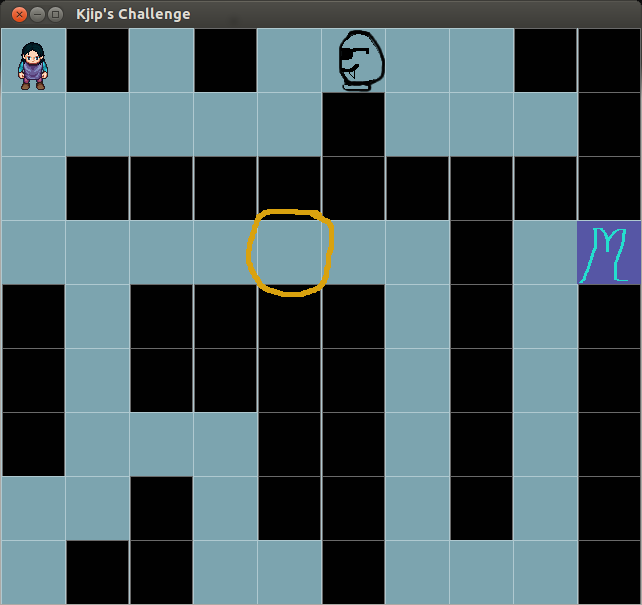
\includegraphics[width=1\textwidth]{eksempel-pa-brett.png}
  \end{figure}
\item [game.entity.types] De forskjellige typene entiteter. Her er kun interface, og ikke noen implementerende klasser.
\item [game.io] Har klasser som snakker med disk og evt. andre programmer som en SQL-database.
\item [game.util] Har forskjellige hjelpemetoder, som Direction for retninger, og Movement for hjelpemetoder til bevegelser.
\item [game.view] Har GameWindow-klassen som er en JFrame som holder på et lerret\footnote{Canvas}. Et lerret er en klasse for å tegne til en flate, som for eksempel en JFrame.
  I tillegg til metoder for popups, kan du også legge til kode om du vil ha mer GUI.
\item [game.view.gfx] Hvor grafikken blir tegnet. Det er også en klasse for å laste bildefiler inn til grafikkmotoren. Dere trenger ikke endre noe her. % Den ene klassen som kan være relevant å se nærmere på er SpriteLoader som er ansvarlig for å laste bildefiler til grafikksystemet.
\item [game.main] Inneholder utelukkende Main, en klasse som er inngangspunktet\footnote{entry-point} for programmet. Det er bare denne klassen i koden dere får som har en main-metode.
\end{description}

%TODO: Få dette renskrevet og inn ordentlig: \\
%Dere skal redigere  game.view.GameWindow, game.controller.Game og game.entity.TileLevel. \\
%Skal lage: game.io.ResourceLoaderSQL og i pakken game.entity.monster.\\
%Det er TODO annotasjoner i relevante kodebiter.   
\section{Oppgaven}
Oppgaven dere skal gjøre kan deles inn i to hoveddeler: Databasebruk og Monstre. Det er også noen ekstrating dere skal gjøre.

\subsection{Utvidelse til bruk av SQL}
\label{subsec:sqloppgave}
Dere skal bruke databaser i dette spillet, nærmere bestemt Apache Derby, som kjører som en del av programmet deres, så dere slipper å tenke på innlogging og slikt. % Som VPN for å bruke MySQL serverene til UiB.
Bibliotekene dere trenger kommer med prosjektet, og er lagt til under lib/ mappen, og satt opp i prosjektet.

\subsubsection{ResourceLoaderSQL}
\label{subsec:resourceloadersql}
Prosjektet har et interface ResourceLoader som beskriver hvordan en klasse kan holdes ansvarlig for å laste inn ressurser fra disk,
som blir implementert av klassen ResourceLoaderCSV.
ResourceLoaderCSV leser dataene fra 4 spesifikke .csv\footnote{CSV - Comma Separated Values} filer og henter inn data derfra.
Vi vil at dere skal implementere en ny klasse ResourceLoaderSQL som bruker en SQL basert database til å hente ut data fra.
For at dette må til bør dere gjøre følgende
\begin{enumerate}
\item Se igjennom .csv filene. Dere kan åpne dem i teksteditorer som Vim og Emacs, eller regneark som MS Excel eller LibreOffice Calc.
\item Finn ut av hva datatypene er, og hvordan disse kan overføres til SQL.
\item Finn ut av hva relasjonene er, og hvordan disse blir vedlikeholdt.\footnote{For eksempel, se på alias.csv og standard-tiles.csv}
\item Når dere nå har modellert en database, da, og først da bør dere skrive koden.
\item Og når dere har skrevet koden, sjekk at den virker.
\item Så kan dere begynne å legge dataene inn i databasen.
\item Og nå når dataene er i databasen, og dere vet at den virker, da bør dere skrive ResourceLoaderSQL klassen.
\item Nest sist, bytt ut ResourceLoader loader = new ResourceLoaderCSV(); med ResourceLoader loader = new ResourceLoaderSQL();
\item Til slutt, fiks alle feil som kommer.
\end{enumerate}

Det er noen viktige ufravikelige krav til ResourceLoaderSQL:
Når dere starter opp spillet skal alle data som trengs fra databasen lastes inn med en gang.
Dere må derfor lagre data i kjøretidsminnet for å unngå at dataene må lastes på nytt.
Dere bør absolutt bruke Map\footnote{se \url{http://docs.oracle.com/javase/7/docs/api/java/util/Map.html}} til å holde på disse dataene, og se på hvordan ResourceLoaderCSV gjør det.
Dere trenger ikke å lagre brettene i relasjonsdatabasen, de kan lagres som tekstfiler slik de er nå. Bildene skal heller ikke ligge i databasen. (Se avsnittet om brettene \ref{subsec:filformat} for mer info.)

\subsubsection{HighScore}
\label{subsec:highscore}
HighScore tabell skal lagres, og når du kommer i mål skal den skrives ut, med spilleren sin plassering vist.
\begin{figure}[h!]
  \caption{En mulig måte å vise highscore på. (Tatt fra SkiFree)}
  \centering
    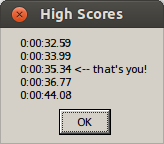
\includegraphics[width=0.5\textwidth]{Mulig-HighScore.png}
\end{figure}

Score i denne sammenhengen er ikke mer komplisert enn antall tidels sekunder brukt, jo færre jo bedre.
Dere må altså lage en ny databasetabell som holder orden på slikt, og tilhørende spørringer for å hente ut informasjon.

\subsection{Monstre}
\label{subsec:monster}
I prosjektet nå er det kun et monster som går en tilfeldig retning. Dere skal lage flere av de klassiske monstrene.
I tillegg til å designe klasser for monstre skal dere også legge til en måte å lagre monsterinformasjon på i databasen.
Dere må både lage en tabell for monstertypene, og en som binder monstre til brett i en mange-til-mange-tabell. Denne mange-til-mange-tabellen må si hvilket monster det er snakk om, hvor på kartet den skal være og hvilket brett det er snakk om.
Monstrene dere skal lage\footnote{Dere kan godt begynne med monstre, og putte dem inn i TileLevel istedenfor ExampleMonster. Se linje 119 i game.entity.TileLevel}\\

Monstrene dere skal lage er:
\begin{description}
\item [VenstreMonster] Dette monsteret går oppover til det treffer et hinder. Da snur det til venstre, og går den veien istedenfor.
\item [HøyreMonster] Dette monsteret går oppover til det treffer et hinder. Da snur det til høyre og går den veien istedenfor.
\item [OppNedMonster] Går opp til det treffer en hindring. Da går det ned til det treffer en hindring. Og slik fortsetter det.
\item [VenstreHøyreMonster] Går til venstre til det treffer en hindring til det treffer en hindring. Når monsteret treffer en hindring snur det $180\,^{\circ}$ og går den veien istedenfor.
\item [MålsøkendeMonster] Går alltid ett steg nærmere spilleren. Skal ikke planlegge en rute men bare gå den ruten som tar den nærmere spilleren.
\item [PatruljeMonster] Følger en gitt patrulje. En patrulje er en streng med en av fire tegn i. N for nord, W for vest, E for øst og S for sør.\footnote{Siden resten av koden er på engelsk følger vi samme praksis her.} Når den har fulgt alle stegene i patruljen begynner den forfra igjen. En patrulje på ``NNEESSWW'' skal gå rundt i ring, for eksempel.
\end{description}

Dessuten skal dere lage en måte å representere monstre på i databasen, og dere utvide må utvide TileLevel til å behandle flere monstre på brettet.

I tillegg må dere kalle metoden tick() på alle monstre i TileLevel.
Når dere kaller tick() kan monstrene gjøre en handling.
Tick blir kalt 120 ganger i sekundet.
Dersom dere gjør noe ved hver mulighet, vil monstrene bevege seg altfor fort.
Se eksempelmonster på en mulighet til å begrense hastigheten.
Når dere kaller tick, skal monstrene bevege seg i prioritert rekkefølge.
Det betyr at dersom du har to monstre med forskjellig prioritet, skal den med høyest prioritet gå først.
Dersom de har samme prioritet betyr ikke rekkefølgen noe.

Her bør dere bruke en prioritetskø\footnote{se \url{http://docs.oracle.com/javase/7/docs/api/java/util/PriorityQueue.html}}.

\section{terminologi}
\subsection{Game-loop}
\label{subsec:game-loop}
En game-loop er en uendelig løkke, og er tradisjonelt delt inn i to:
\begin{description}
\item [oppdatering] Oppdaterer tilstanden til alle objekter i spillet. Blant annet ting som å sjekke om spilleren har dødd, lese ting fra tastaturet, og la datastyrte entiteter som monstre bevege seg.
\item [tegning] tegner verdenen spilleren skal se etter opppdatering.
\end{description}
I spillet dere skal utvide er løkken forenklet, ved at tastaturinput og tegning er gjort for dere.
Det er altså kun oppdatering som skjer i løkken, tegning skjer i en annen tråd.

\subsection{Tick}
\label{subsec:tick}
Et tick er en sjanse for en skapning til å velge å gjøre en ting.
Dersom du for eksempel får 4 ticks i sekundet kan ikke en AI\footnote{AI = kunstig intelligens. Se \url{http://no.wikipedia.org/wiki/Kunstig_intelligens}} reagere raskere enn 1/4 sekund.
Bare fordi du får mange ticks betyr ikke at en AI må bruke alle. Den kan utmerket godt kun bevege seg annenhver tick, eller sjeldnere.
I vårt spill har alle klasser som implementerer Tickable-interfacet en tick() metode som er void, og lar objekter av den klassen oppdatere seg selv når metoden blir kalt.

\subsection{Sprite}
\label{subsec:sprite}
En sprite er et mulig bilde av en entitet eller en del av en entitet i et spill.\footnote{På eldre maskiner som den første Nintendoen, var det sterkte begrensede ressurser. En fant ut at dersom en lastet inn flere bilder på en gang som ett stort bilde var det mye raskere for grafikkprosessoren. En kunne også veldig enkelt be om å kun tegne en bit av bildet. Tradisjonen med å samle bilder fra samme entitet på et sted ble da født. En kunne også modde for eksempel det første GTA spillet med å åpne opp spritesheets og tegne om på ting.}
I Kjips Kylling er for eksempel spilleren som ser ned en sprite. Det er tre andre sprites som brukes om spillerfiguren, nemlig når den ser opp, til venstre eller til høyre.
En gulveflis har bare en sprite, siden den ikke kan snu seg til venstre.
\subsection{Spritesheet}
\label{subsec:spritesheet}
En spritesheet er en bildefil som inneholder mange sprites samlet i en fil. Ble opprinnelig brukt for å spare på systemressurser, og blir fortsatt brukt på internett av den grunn.
(Hvis du har mange bildefiler som må sendes over serveren må du motta og behandle mange kall. Dersom bildefilene er små bruker du plutselig mer tid på å behandle kallene enn på å sende informasjon.
Men dersom du samler alle de små bildene sammen i ett bilde og sender det, og deretter sakser ut biter av bildet til nettsiden din, går alt mye fortere.
Vi som har såpass små bildefiler kunne utmerket godt sluppet unna med å ha separate bildefiler, men vi valgte å ha det med, fordi det er enklere å se hvordan bildene ser ut, mindre File objekter å skyfle rundt på, for å følge tradisjonen, og fordi det er greit å ha sett hvis du i fremtiden skal lage nettsider.
Se \url{http://css-tricks.com/css-sprites/} hvis du lurer på hvordan det brukes i nettsider.

\subsection{Filformater}
\label{subsec:filformat}
Dere trenger ikke røre hverken brettfiler eller spritesheets, men dere kan hvis dere vil. Her er derfor en oversikt over filformatene.
\subsubsection{Spritesheets}
\label{subsec:spritesheet-file-format}

Det er fire forskjellige spritesheets i prosjektet, og ligger i undergruppen art/.
\begin{description}
\item [figur.png] Er spriten til hovedpersonen. Den er laget vha. \url{gaurav.munjal.us/Universal-LPC-Spritesheet-Character-Generator/}, og dere kan lage deres egen figur der.
  Den har mange tilstander som kan brukes, men vi bruker bare fire av dem.
  Dersom du lager en ny bildefil i siden du vil bruke, bør du først gi figur.png et nytt navn, og så gi den nye filen navnet figur.png etterpå.
\item [Sara.png] Er maskoten til opengameart. Dere kan bruke den istedenfor figur.png hvis dere vil, da de har samme format.
\item [monstre.png] Er en spritesheet med flere monstre på. Hvis dere vil modde monstrene til å se annerledes ut, kan dere redigere den filen.
\item [tiles.png] Er spritesheeten for rutene på kartet. Endrer dere på dette bildet endrer dere hvordan flisene blir tegnet.
\end{description}
Tilesheets er forventet å legge under art/ undermappen. Selv om du kan registrere tilesheets andre steder, anbefales det sterkt at dere følger konvensjonen.
\subsubsection{CSV-filene}
\label{subsec:csv-filene}
CSV er et filformat som forenklet sett beskriver en todimensjonal tabell.
Hvert felt i en rad er adskilt med komma, med en mulig overskrift som beskriver tabellen.
Dette er nok til å beskrive alle csv-filene i oppgaven.
Hvis dere vil lese mer om CSV, kan dere se på\url{http://en.wikipedia.org/wiki/Comma-separated_values} for generell informasjon, og \url{http://tools.ietf.org/html/rfc4180} for en spesifikasjon.

\begin{description}
\item [adventure.csv]      beskriver hvilke brett som skal spilles, med rekkefølge, navn på brettet og til slutt hvor brettfilen finnes.
\item [spritesheets.csv]   beskriver hvilke spritesheets som skal lastes inn, med deres navn, plassering av filen, og størrelsen på et bilde (tilesize) i piksler.
\item [standard-tiles.csv] beskriver vanlige ruter i et brett, med navn, om spilleren skal kunne gå på dem, om spilleren dør om den betråkkes, og hvor i spritesheeten den er (kolonne og rad som to felt).
\item [alias.csv]          beskriver aliaser, altså hvilke bokstaver som betegner hvilke ruter, med tegnet, og så navnet på ruten.
\end{description}

\subsubsection{Brettfilene}
\label{subsec:brettfil}

En brettfil er en vanlig tekstfil, og består av følgende:
Først seks heltall på en linje.
\begin{enumerate}
\item Hvor mange kolonner som er i brettet
\item Hvor mange rader som er i brettet
\item Hvilken kolonne spilleren begynner på
\item Hvilken rad spilleren begynner på
\item Hvilken kolonne spilleren skal begynne på
\item Hvilken rad spilleren skal ende på
\end{enumerate}
Så følger en rekke linjer med enkelttegn, et tegn for hver kolonne, en linje for hver rad.
Hvert tegn svarer til en rute, som definert i alias.csv. (Disse definisjonene skal selvsagt over i den relasjonelle databasen.)
\end{document}
